\documentclass[10pt]{article}

\usepackage[T1]{fontenc}
\usepackage{lmodern}
\usepackage[letterpaper,margin=0.75in]{geometry}
\usepackage{graphicx}
\usepackage{xcolor}
\usepackage{caption}
\usepackage{hyperref}

\graphicspath{{figures/}}
\captionsetup{font=small,labelfont=bf}
\definecolor{egfnblue}{HTML}{2878B5}
\hypersetup{
  colorlinks=true,
  linkcolor=egfnblue,
  urlcolor=egfnblue,
  pdftitle={Energy-Gated Frequency Networks: Supplementary Material},
  pdfauthor={Henry}
}

\title{\textbf{Energy-Gated Frequency Networks}\\Supplementary Material}
\author{Henry}
\date{July 2026}

\begin{document}
\maketitle

This supplement preserves diagnostic figures removed from the compact main
paper. They document the historical model progression but do not resolve the
causal contribution of gating. Reported validation values are descriptive
results from development experiments.

\section{Filter-bank evolution}

The hard synthetic task motivated a progression from five coarse fixed filters
to eight fixed filters and then to free FIR kernels. The free kernels improved
validation accuracy, but their spectral responses became irregular and
multi-band. Consequently, initialized band names are not physical guarantees
after unconstrained learning.

\begin{figure}[ht]
\centering
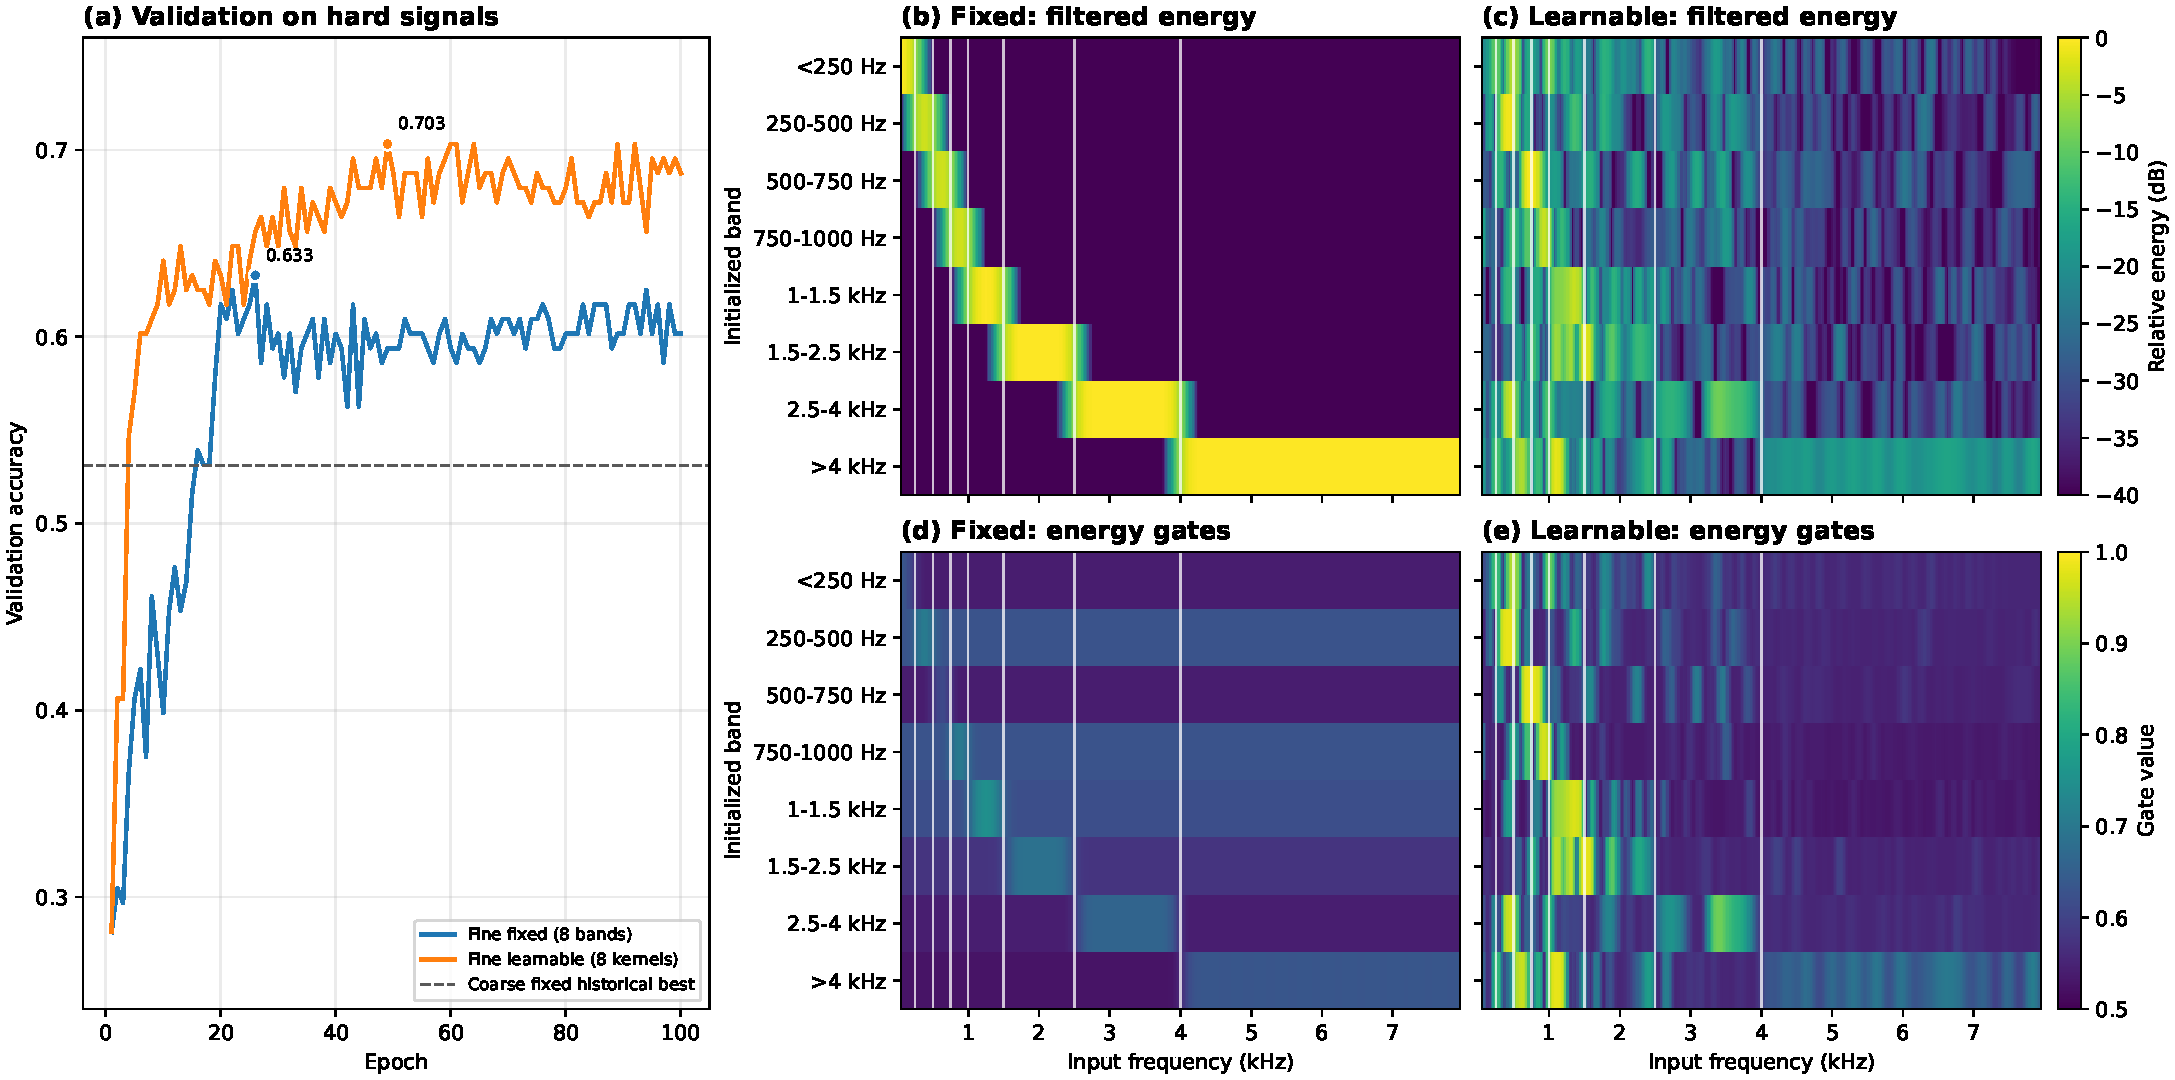
\includegraphics[width=0.98\textwidth]{fig03_filter_evolution.pdf}
\caption{Evolution from coarse fixed filters to a fine fixed bank and free FIR
kernels. Free kernels improve the hard-task result while weakening explicit
low-pass, high-pass, and band-pass interpretation.}
\end{figure}

\clearpage
\section{Gate variants}

Independent, contextual, and sparsity-regularized gates were compared on the
hard synthetic validation split. Nearly all gates remained above $0.5$; a low
mean activation or a threshold-dependent active-band count should therefore not
be interpreted as proof of discrete routing.

\begin{figure}[ht]
\centering
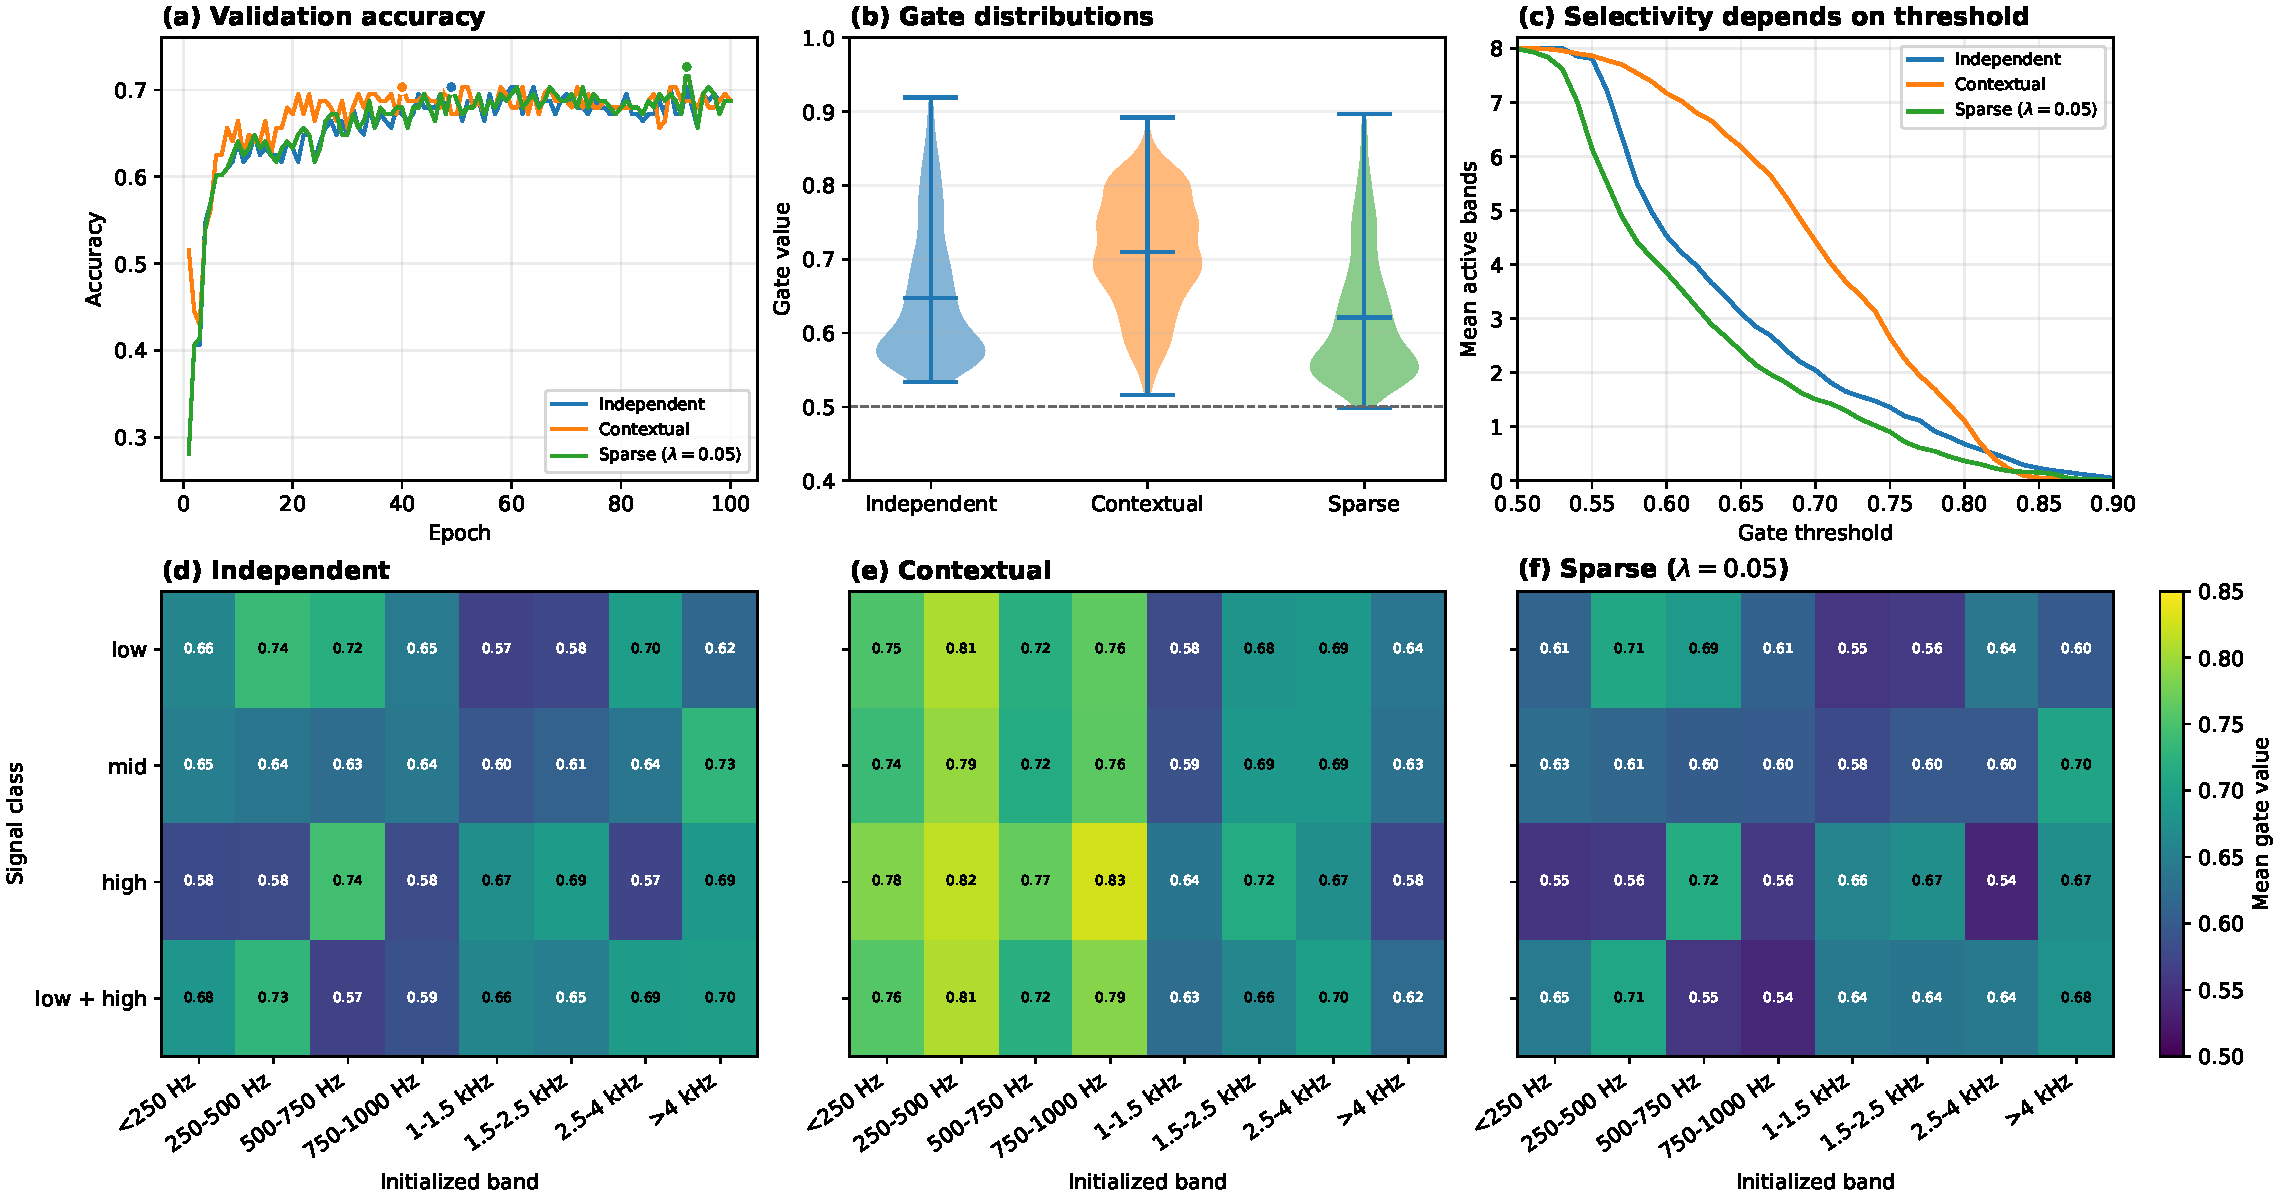
\includegraphics[width=0.98\textwidth]{fig04_gate_evolution.pdf}
\caption{Independent, contextual, and sparsity-regularized gate behavior. The
results support soft attenuation, not hard feature selection.}
\end{figure}

\clearpage
\section{FSDD split sensitivity}

A random recording split contains voices observed during training, whereas the
speaker-disjoint protocol evaluates an unseen voice. The large performance gap
shows that the random split cannot be used as evidence of speaker invariance.

\begin{figure}[ht]
\centering
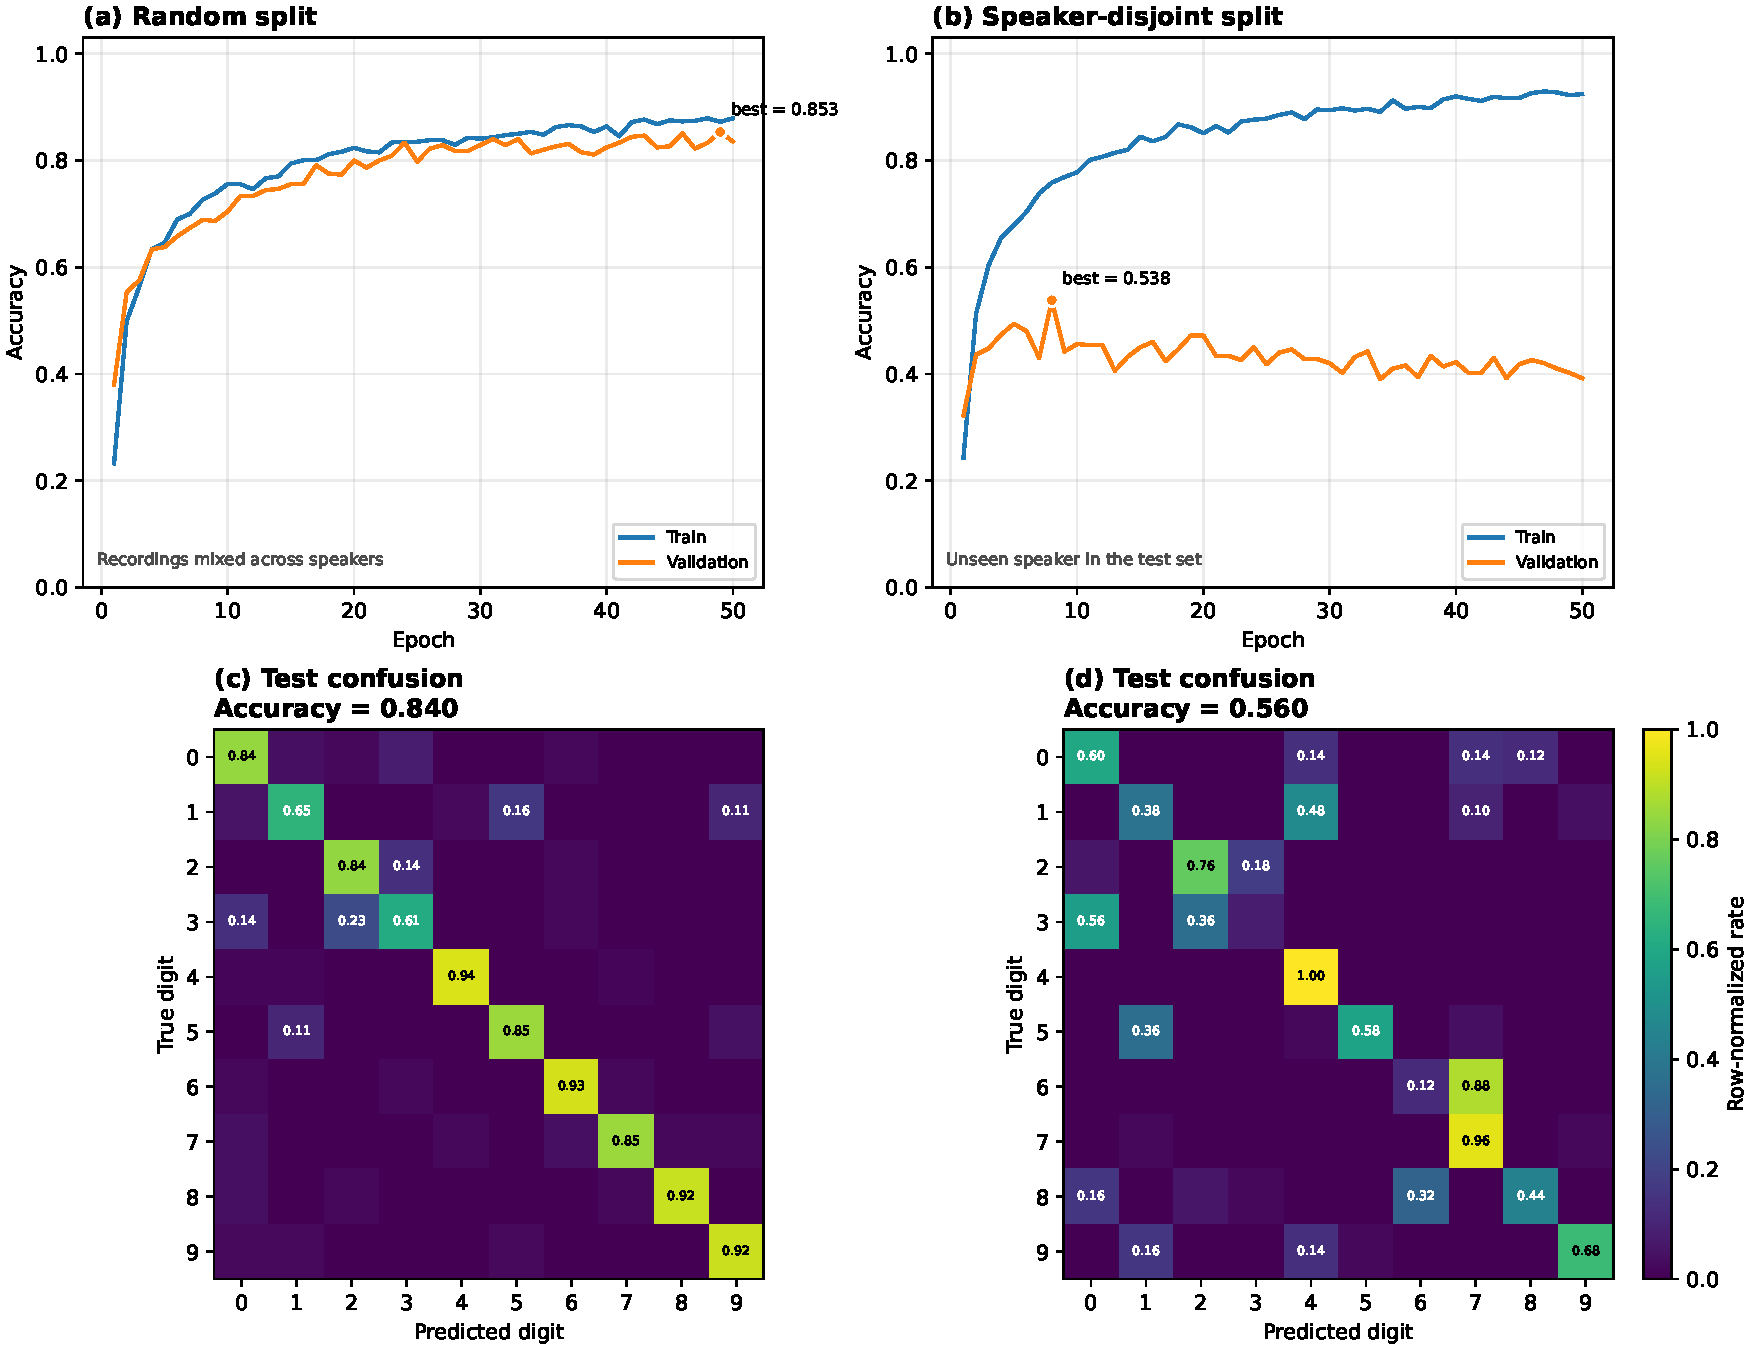
\includegraphics[width=0.98\textwidth]{fig05_fsdd_splits.pdf}
\caption{Random versus speaker-disjoint FSDD evaluation, including training
histories and normalized confusion matrices.}
\end{figure}

\clearpage
\section{FSDD temporal head comparison}

Replacing global pooling with a temporal head recovered $14.8$ percentage
points on the speaker-disjoint test, but Conv1D retained the best test accuracy
with fewer parameters than Temporal EGFN. This result supports the importance
of temporal order rather than an isolated advantage of the frequency frontend.

\begin{figure}[ht]
\centering
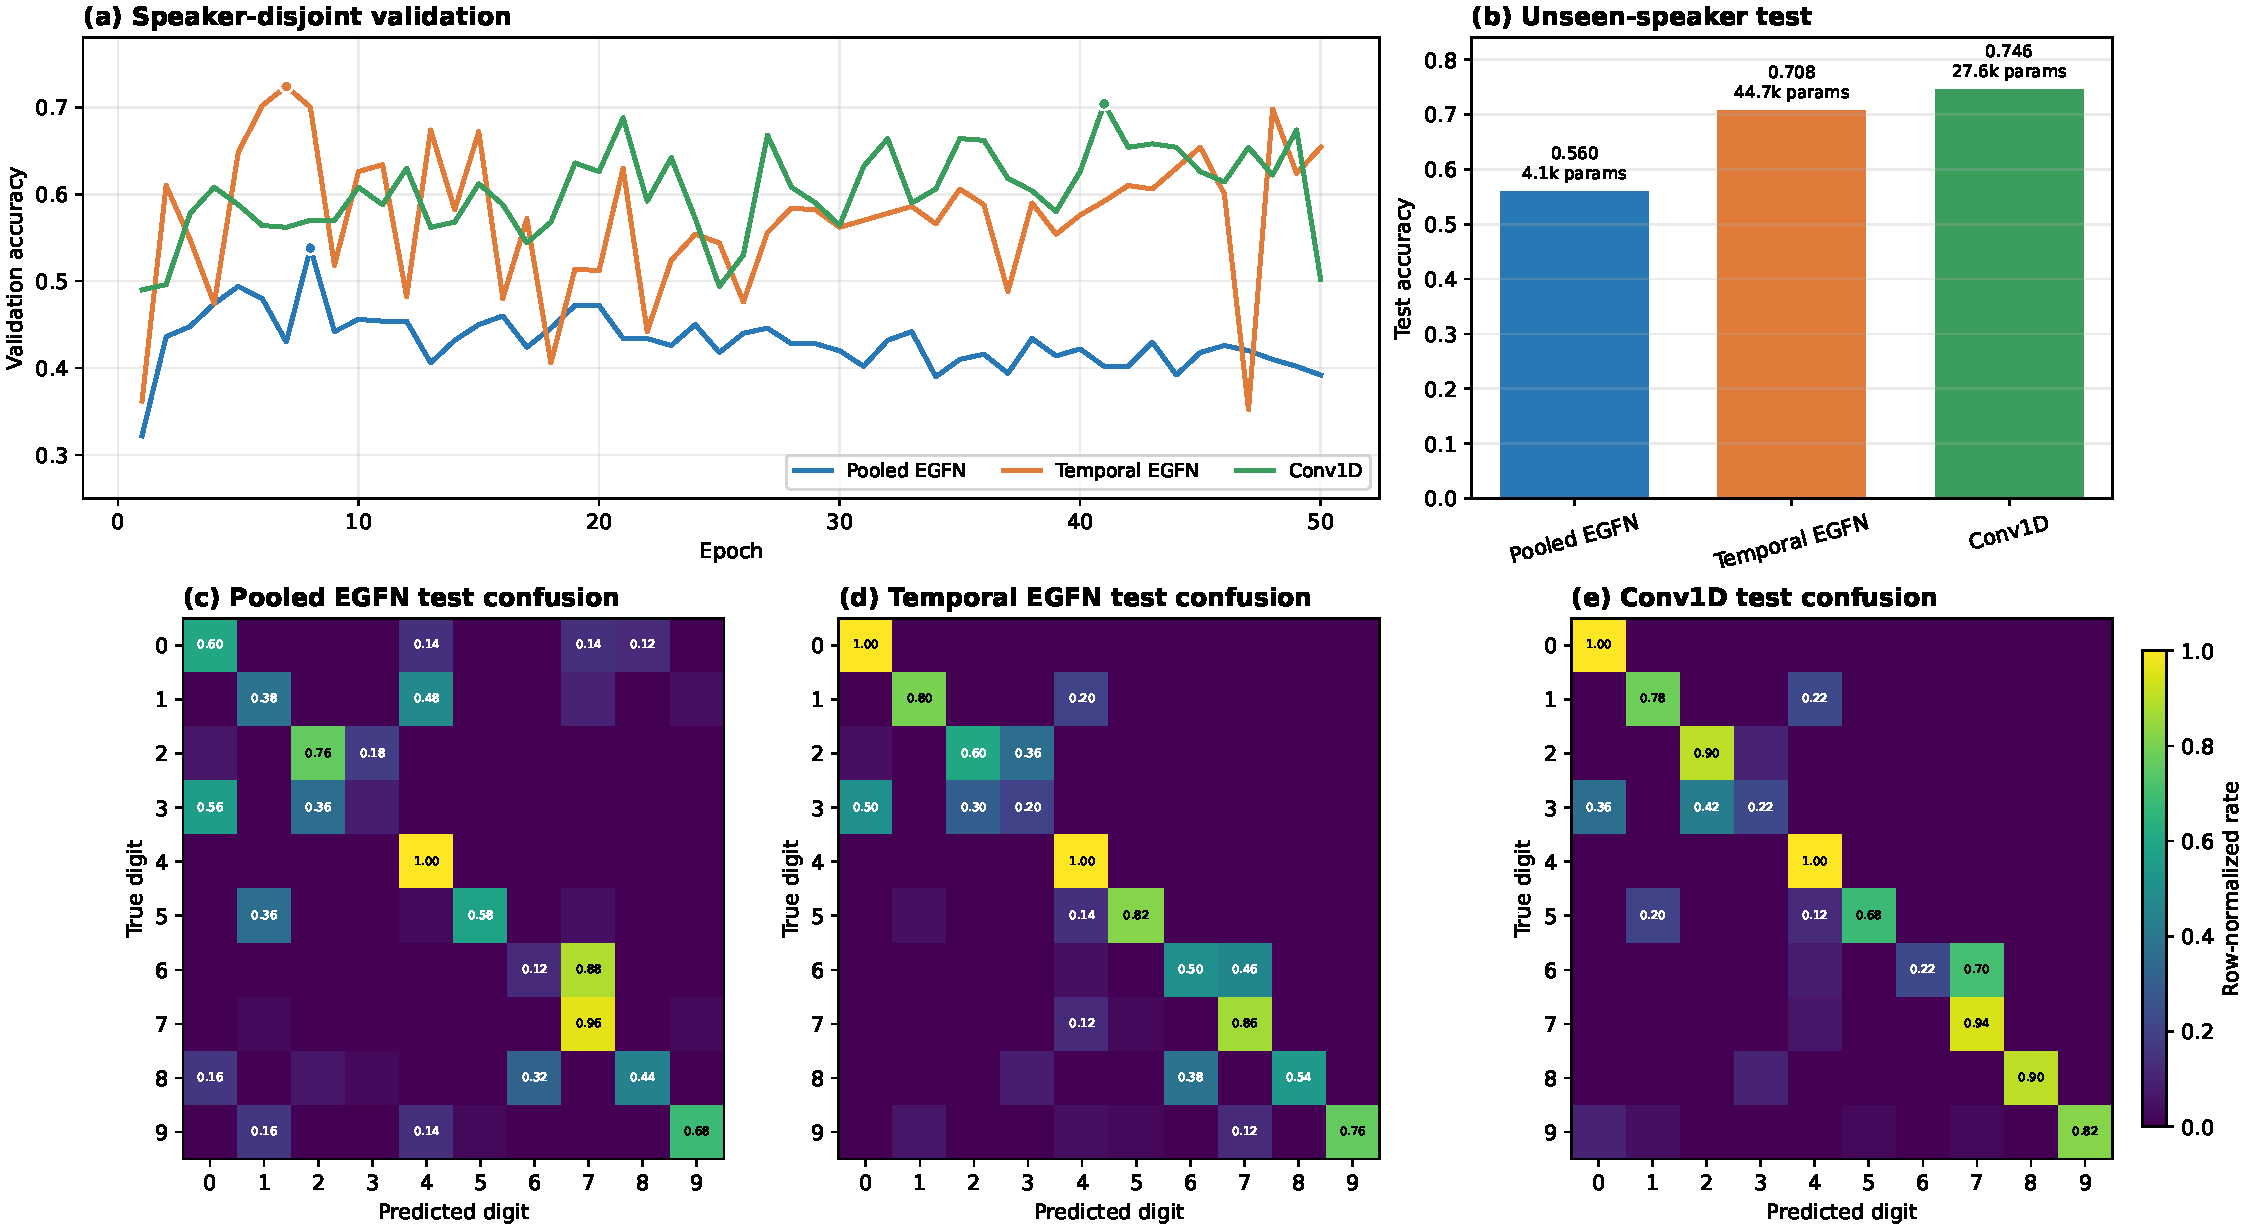
\includegraphics[width=0.98\textwidth]{fig06_fsdd_temporal.pdf}
\caption{Pooled EGFN, Temporal EGFN, and Conv1D under speaker-disjoint FSDD
evaluation.}
\end{figure}

\end{document}
